\section{Data-dependent, quantity-optimized streams}
\label{sec:data_dep_streams}

This section aims to solve the problem of finding the most optimal (and data-dependent) stream
possible, given a data set and an error metric. An error metric is a function $E(Q(f'),Q(f))$, where
$f$ is the original data field and $f'$ is a reconstructed version of $f$ using a subset of the
bits. $Q$ is an operation that trasnforms a raw data fields (e.g., $f$ and $f'$) to some quantity of
interest (e.g., derivatives, histograms, isocontours, etc). There can be multiple error functions
$E$ that makes sense for the same quantity $Q$. In this paper, we choose to use only one error
metric with each quantity, one which we believe is either common, or intuitive and simple without
sacrificing generalizability. The list of quantity-optimized streams studied in this paper includes
\emph{rmse-optimized} (Section [REF]), \emph{gradient-optimized} (Section [REF]),
\emph{laplacian-optimized} (Section [REF]), \emph{histogram-optimized} (Section [REF]), and
\emph{isocontour-optimized} (Section [REF]).

Studying a (data-dependent) quantity-optimized stream is important because such a stream serves both
as a benchmark, and a source of insights for other, more practical streams for the same quantity.
One way to define the ``optimal'' stream for a quantity $G$ could be the stream that incurs the
minimum error $E$ at every point. However, in trying to realize it, our experience has been that
such a stream does not exist. Assume otherwise that the optimal stream exists, then by its
definition, it must be possible to construct it using the following greedy algorithm: start with a
pool of all the chunks (and correspondingly an all-zero $f'$ and a presumably very high $E$), pick
the chunk that when enabled, would minimize $E$, remove it from the pool. Repeatedly pick the next
chunk that minimizes $E$, until the pool is empty. Running this algorithm, we have noticed that
there can be a situation in which the next chunk that minimizes the error is on a low-order bit
plane of a very fine-scale coefficient, which contributes little to the reconstructed function. The
error is minimized because it is kept approximately constant. In this case it is actually better to
pick a chunk that increases the error, but otherwise contributes a lot more to the reconstructed
function. In optimization terms, it is necessary to move in a direction that increases the error to
avoid getting stuck in a local minima.

The optimal stream for an error metric can also be defined as the stream such that the area bounded
by its plotted error curve and the horizontal axis is smallest. However, the usefulness of such a
definition is limited in practice, because a stream should be able to be terminated at any point and
still be expected to produce as small of an error as possible. Instead, we observe that the greedy
algorithm stated in the paragraph above can be slightly modified to avoid the problem of being stuck
in local minima. We start with a pool consisting of all the chunks and an empty stream, and build
the stream back to front. In each step, the chunk whose removal from the pool has the least impact
on the error $E$ is removed and inserted to the beginning of the current stream. This algorithm
solves the problem of unimportant chunks being picked too early in the original algorithm, because
here, being picked early means they would be at the end of the stream, instead of the beginning.

In our experience, however, the back-to-front greedy algorithm is too costly in practice. Ignoring
all the steps done in each iteration, this algorithm amounts to an $n^2$-iteration, 2-level nested
loop, where $n$ is the number of chunks. In 2D, with a $256^2$ data set, a chunk size that spans
$16$ coefficients, and $16$ bits of quantization, the total number of chunks would be $n=65536$, and
$n^2$ would be in the billions, which we have found to be prohibitively large. We have therefore
adopted a simplified version of this algorithm, where only one pass through the chunks are needed.
Our modified algorithm disables (sets to zero) a new chunk $c_i$ in each iteration, computes and
records the error $E_i$ due to chunk $c_i$ missing, and enables again the chunk at the end of the
iteration. After $n$ iterations, each chunk has an associated weight, $E_i$. The optimal stream,
then, is simply a sorted list of chunks, in decreasing order of the weights. In our experience, this
simplified algorithm brings the running time down from days to minutes, while retaining the same
performance.

\textbf{Minimizing function error in $L_2$} The most fundamental task is that of reconstructing the
function itself (i.e., $Q$ is the identity map), using a common error metric such as the
root-mean-square error (RMSE). For each data set, we use the aforementioned $O(n)$ greedy algorithm
to construct an \emph{rmse-optimized} stream. In Section \ref{sec:motivation} we have seen that the
\emph{by wavelet norm} performs the best among the data-agnostic streams with regards to RMSE. To
see how the \emph{rmse-optimized} stream, which is data-dependent, compares to the data-agnostic
streams, we plot all four streams together in Figure \ref{fig:rmse-optimized}. It can be seen that
the difference between \emph{by wavelet norm} and \emph{rmse-optimized} is negligible. This result
is expected, because \emph{by wavelet norm} and \emph{rmse-optimized} both order the chunks
according to their contribution to the function in $L_2$ sense, with \emph{rmse-optimized} taking
into account the actual values of the bits. This difference has little effect in this case, because,
as leading zero bits are removed, the rest of the bits (of the wavelet coefficients) are known to be
distributed approximately uniformly among $0$ and $1$ for wavelet coefficients [CITE]. These results
suggest that in practice, \emph{by wavelet norm} is a near-optimal way to stream data that minimizes
root-mean-square errors, regardless of the data.

\begin{figure}
  \centering
	\subcaptionbox{Boiler}
  {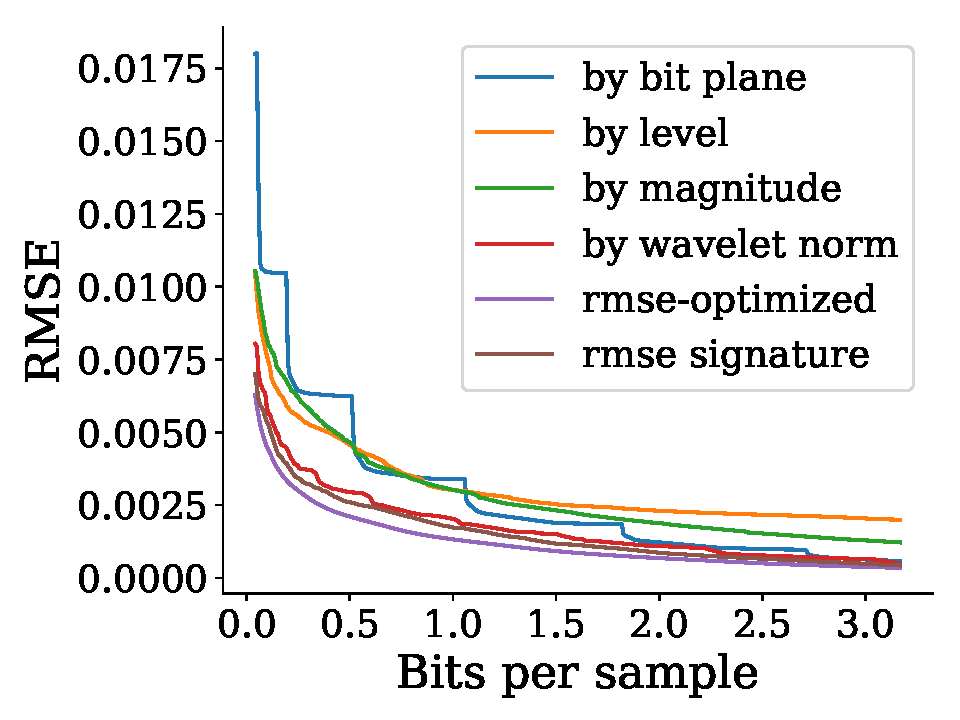
\includegraphics[width=0.48\linewidth]{img/rmse/rmse-optimized-boiler.pdf}}
	\subcaptionbox{Diffusivity}
 	{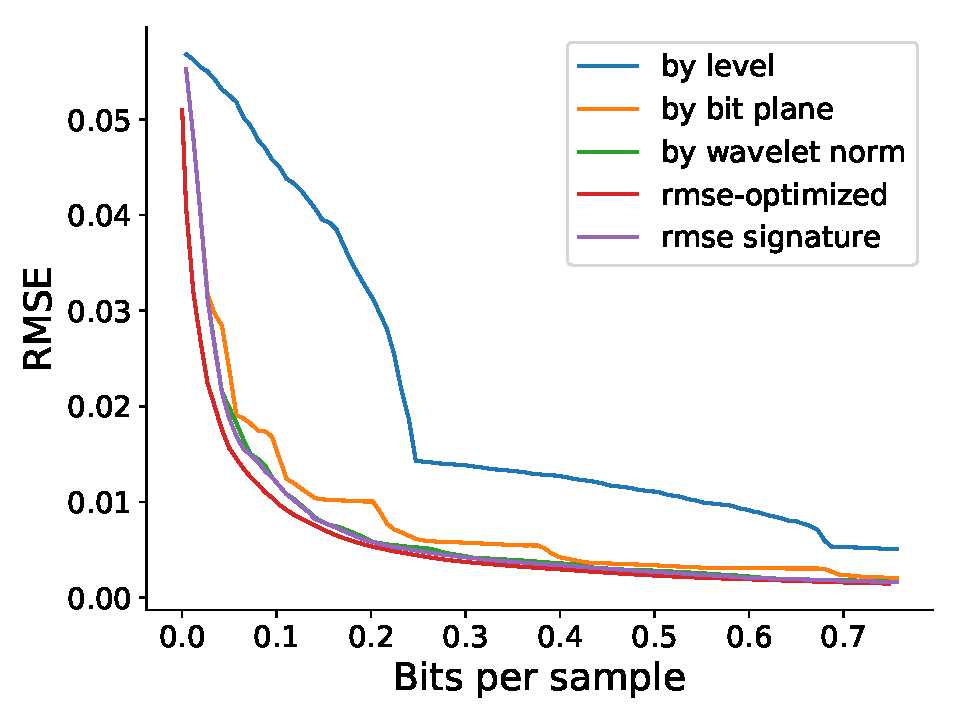
\includegraphics[width=0.48\linewidth]{img/rmse/rmse-optimized-diffusivity.pdf}}
	\subcaptionbox{Euler}
 	{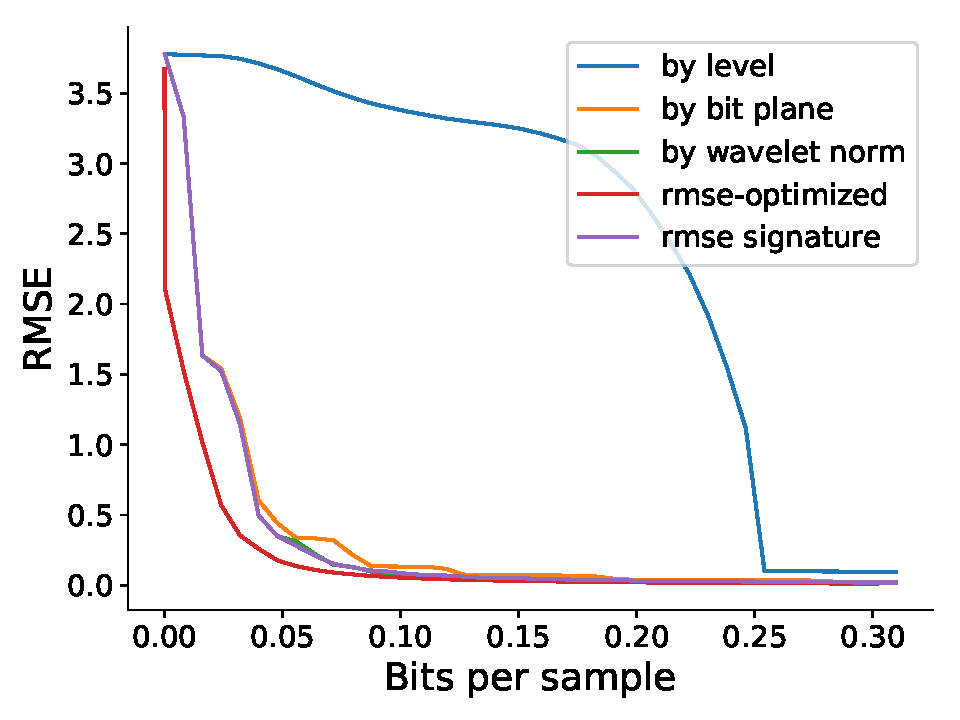
\includegraphics[width=0.48\linewidth]{img/rmse/rmse-optimized-euler.pdf}}
	\subcaptionbox{Turbulence}
 	{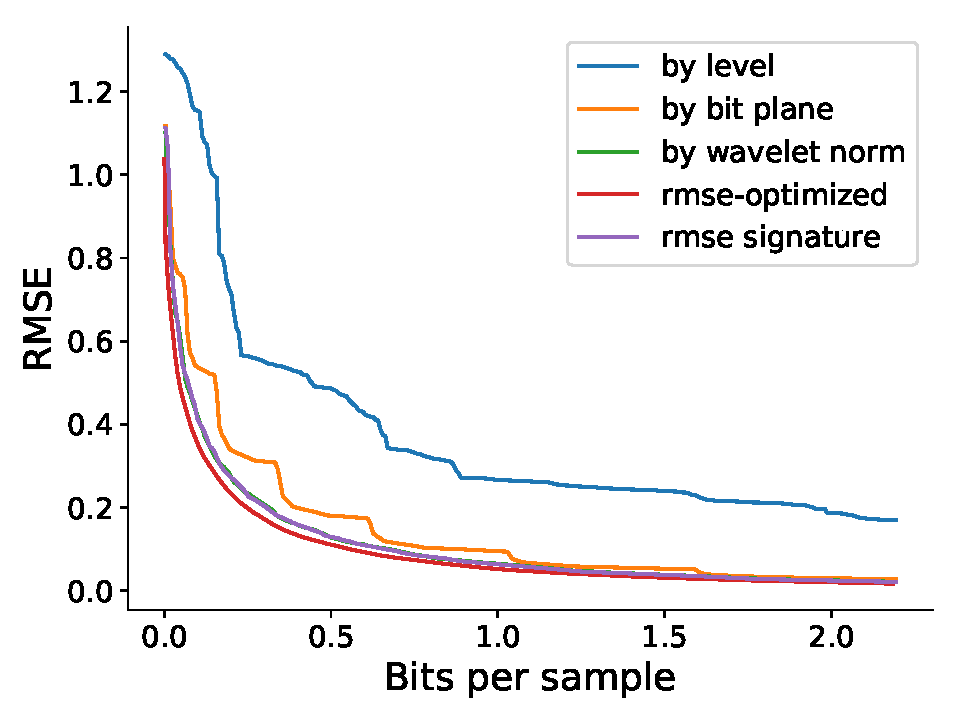
\includegraphics[width=0.48\linewidth]{img/rmse/rmse-optimized-turbulence.pdf}}
	\subcaptionbox{Plasma}
 	{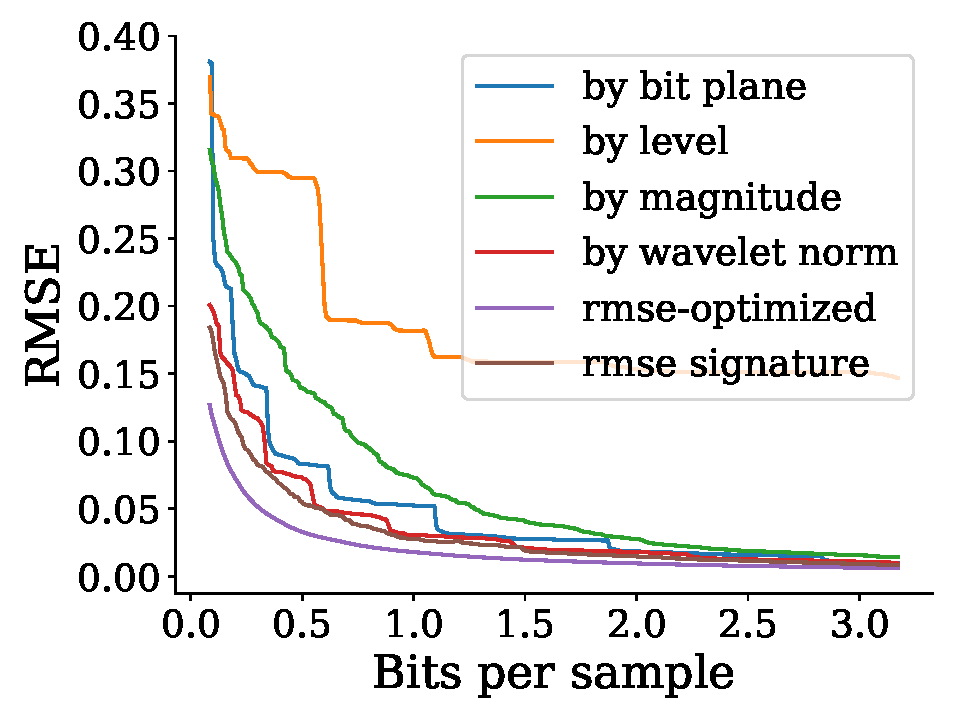
\includegraphics[width=0.48\linewidth]{img/rmse/rmse-optimized-plasma.pdf}}
	\subcaptionbox{Velocity-z}
 	{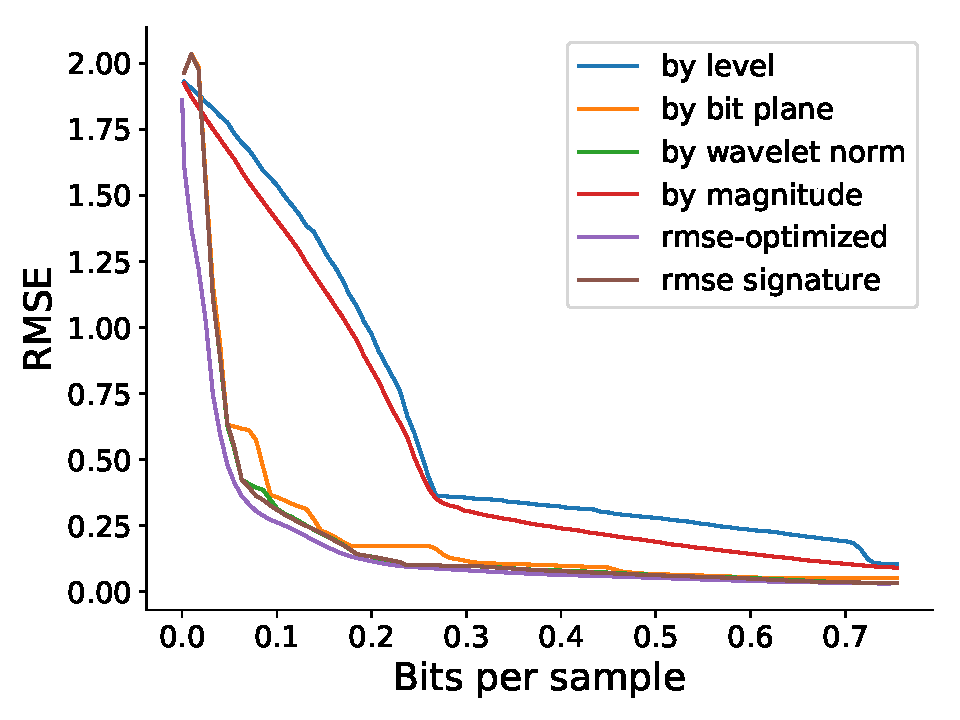
\includegraphics[width=0.48\linewidth]{img/rmse/rmse-optimized-velocityz.pdf}}
 	\caption{Root-mean-square error of reconstructed functions for the three data-agnostic streams
 	defined in Section \ref{sec:motivation}, and the \emph{rmse-optimized} stream. Lower is better.
 	The streams are truncated to highlight the differences, without omitting important information.
 	\emph{rmse-optimized} performs best, followed closely by \emph{by wavelet norm} and \emph{by bit
 	plane}.}
 	\label{fig:rmse-optimized}
\end{figure}

TODO: add renderings of data for comparisons
